\chapter{让路点之间更平顺：二维 MINCO}
\begin{notebox}
\textbf{目标}\quad 给定路点和时长求最小 jerk 曲线，把系数代价传回路点与时长。\\
\textbf{先修}\quad 第 14 章；矩阵方程、链式法则，本章补充必要的最优化条件。
\end{notebox}

\section{相同路点、相同时长的比较}
\begin{lstlisting}[language=bash]
ros2 run motion2d minco_demo tmp/ch15_minco
/usr/bin/python3 scripts/plot_ch15_minco.py
\end{lstlisting}
上一章在每个路点停下，易于构造，但未选择合适的中间速度和加速度。
本章固定路点 $q_i$ 与分段时长 $T_i>0$，保留两端的 p/v/a，求解整个区间的
\begin{equation}
\min J=\sum_{i=1}^{N}\int_0^{T_i}\|p_i'''(t)\|^2\,dt.
\end{equation}
jerk 是加速度的变化率。$J$ 常被称为控制能量，这里单位是 $\mathrm{m^2/s^5}$，不是物理焦耳。
MINCO 是一种利用路点和时长确定最小控制代价轨迹的表示；课程根据
\href{https://arxiv.org/html/2103.00190v4}{作者论文}中的最优性思想，独立实现固定二维、五次、最小 jerk 子问题。

\begin{figure}[!ht]
\centering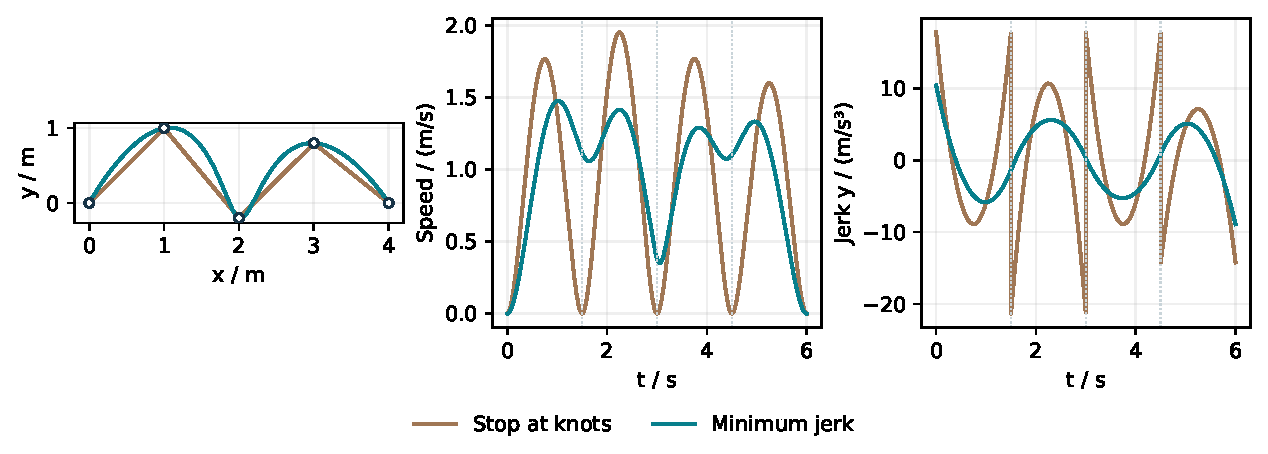
\includegraphics[width=\linewidth]{figures/ch15_minco.pdf}
\caption{四段均为 1.5 s。圆点是固定路点，虚竖线是连接时刻。
最小 jerk 解允许内部点有非零速度，连接处 jerk 连续；此图没有施加避障约束。}
\end{figure}

\section{能量是系数的二次型}
将单段系数按升幂排成 $C\in\mathbb R^{6\times2}$，则 $J_i=\operatorname{tr}(C^TQ(T_i)C)$。
$Q$ 只有第 3 到 5 次项对应的部分非零；对 $k,l\geq3$，
\begin{equation}
Q_{kl}(T)=\frac{k(k-1)(k-2)\,l(l-1)(l-2)}{k+l-5}T^{k+l-5}.
\end{equation}
这只是先求导、相乘再积分；代码 jerkGram 没有数值积分误差。
练习 ch15-1 用单段 $J=720\|p_1-p_0\|^2/T^5$ 检查因子与幂次。

\section{为什么最优解还要连续 jerk 与 snap}
只要求 p/v/a 连续时，内部速度和加速度仍可调整。
让曲线发生一个小变化 $\delta p$，对 $\delta J=2\int p'''\cdot\delta p'''dt$ 做三次分部积分，得到
\begin{equation}
\frac{\delta J}{2}=\left[p'''\cdot\delta p''-p''''\cdot\delta p'
+p'''''\cdot\delta p\right]_0^T-\int_0^T p^{(6)}\cdot\delta p\,dt.
\end{equation}
每段内部变化任意，故最优解满足 $p^{(6)}=0$，即至多五次。
在固定位置的内部路点处 $\delta p=0$，而两侧共享的 $\delta v,\delta a$ 可以自由变化。
相邻段端点项的符号相反，因此它们的系数必须抵消：jerk 与 snap 分别连续。
合上原有 p/v/a 连续，便得到 $C^4$；第五阶导数仍可跳变。

\section{将最优性写成一组线性方程}
每段六个系数，每个坐标共 $6N$ 个未知数。方程数量恰好也是 $6N$：
\begin{itemize}
\item 首尾各三个 p/v/a 条件，共 6 行。
\item 每个内部连接：jerk、snap 连续各一行，左段终点固定位置一行，p/v/a 连续三行，共 6 行。
\end{itemize}
把二维系数堆为 $C\in\mathbb R^{6N\times2}$，一次求解两个右端项：
\begin{equation}
A(T)C=B(q).
\end{equation}
每一行只涉及相邻两段，所以按代码顺序排列后，上下带宽均为 6。
\lstinputlisting[language=C++,linerange={minco_conditions_begin-minco_conditions_end},
  includerangemarker=false]{../ros2_ws/src/motion2d/src/trajectory/minco2d.cpp}
insert 将对应阶导数的基函数系数放入矩阵；例如零时刻 jerk 对 $c_3$ 的系数是 6。
矩阵约束已经包含最优性，求解阶段无需再迭代下降能量。trajectory() 返回上一章的统一采样对象。

\clearpage
\section{系数随路点和时长一起变化}
以后添加避障或速度代价，先计算它们对系数、时长的\textbf{直接偏导}。
记 $G=\partial K/\partial C$、$g_T=\partial K/\partial T$；固定系数时，jerk 代价有
\begin{equation}
G_i=2Q(T_i)C_i,\qquad (g_T)_i=\|p_i'''(T_i)\|^2.
\end{equation}
但是改变 $T_i$ 后，保持边界条件需要重新求系数；只保留这个非负上限项，会丢掉关键变化。
例如单段静止到静止的完整导数为 $dJ/dT=-3600\|\Delta p\|^2/T^6$，反而是负值。

对 $AC=B$ 求微分，得到 $A\,dC=dB-(dA)C$。
为了避免对每个路点单独求一次 $dC$，先求一个\textbf{伴随方程}：
\begin{equation}
A^T\Lambda=G,\qquad
 dK=\langle\Lambda,dB-(dA)C\rangle+g_T^T dT.
\end{equation}
$\langle X,Y\rangle=\sum_{ij}X_{ij}Y_{ij}$ 表示逐项乘积求和。
一个路点只改变 $B$ 对应的一行；故直接取该行 $\Lambda$。
某一时长只改变其所在段的右端导数值；再对时间求导，阶数增加一阶。
\lstinputlisting[language=C++,linerange={minco_adjoint_begin-minco_adjoint_end},
  includerangemarker=false]{../ros2_ws/src/motion2d/src/trajectory/minco2d.cpp}
中间连接对应的导数阶数为 $[4,5,1,1,2,3]$，与上一页六行方程逐一对应；
最后一段仅有末端 p/v/a，使用 $[1,2,3]$。
energyPartials 给出直接偏导；propagate 输出总路点/时长梯度，也能处理未来其他可微代价。

\section{为什么不用显式矩阵求逆}
代码先将 $A$ 分解为 $LU$，正向求解先解 $Ly=B$、再解 $UC=y$。
伴随复用同一组因子，先解 $U^Ty=G$、再解 $L^T\Lambda=y$。
固定带宽下，每行只读写常数个邻居，储存、分解和每次求解都随段数线性增长。
这指算法复杂度；实际速度对照在第十六章测量。

\clearpage
\section{带状实现和数值尺度}
\lstinputlisting[language=C++,linerange={band_factor_begin-band_factor_end},
  includerangemarker=false]{../ros2_ws/src/motion2d/src/trajectory/banded_lu.cpp}
BandedLu 只保存每行附近 13 个元素。教学实现使用本章特定顺序的无主元 LU，
不是任意矩阵的通用稳定求解器。若主元非有限或绝对值小于 $10^{-14}$，明确报告数值失败。
正时长保证数学问题可解，不保证任意悬殊尺度下的浮点计算稳定；优先使用秒、米和适中的分段时长。

\section{独立检查比看图更可靠}
测试另建一个密集等式约束二次型：只约束位置和 p/v/a 连接，不加入 jerk/snap 连续条件。
jerk 平方积分用三点 Gauss--Legendre 求积计算，它对该四次被积式精确。
将能量的驻点条件与等式约束联立为密集线性系统（KKT），求解后与带状结果比较，
避免用同一组最优性方程自证。
1--6 段、seed=1515 的小问题，系数相对误差门限为 $2\times10^{-9}$，连接到四阶检查门限为 $10^{-8}$。

对路点和时长采用步长 $10^{-5}$ 的中心差分，检查完整伴随梯度；
测试还增加系数平方与显式时长平方项，避免只验证 jerk 这个特殊目标。
允许误差为 $2\times10^{-6}\max(1,|g_{\mathrm{FD}}|)$，不是用差分替代实现中的解析梯度。

\begin{center}\small
\pgfplotstabletypeset[col sep=comma,
columns={mode,energy,peak_speed,peak_acceleration},
columns/mode/.style={column name=模式,string type,string replace*={0}{逐点停靠},string replace*={1}{MINCO}},
columns/energy/.style={column name=jerk 积分, fixed,precision=3},
columns/peak_speed/.style={column name=速度峰值, fixed,precision=3},
columns/peak_acceleration/.style={column name=加速度峰值, fixed,precision=3},
every head row/.style={before row=\toprule,after row=\midrule},
every last row/.style={after row=\bottomrule}]{data/ch15_minco.csv}
\end{center}
演示两端为 $(0,0),(4,0)$ m，中间为 $(1,1),(2,-0.2),(3,0.8)$ m，首尾静止。
四段各 1.5 s；能量是解析积分，速度/加速度峰值来自 3001 个采样点。
本次能量降低，曲线也偏离折线；\textbf{没有施加障碍、走廊或动力学约束}。

\begin{enumerate}
\item \textbf{推导：}为什么只固定内部位置，最优解仍有连续 jerk 与 snap？
\item \textbf{代码 ch15-1：}完成 jerkGram 的一个条目，检查低次项为零、积分指数和因子。
\item \textbf{实验：}固定相同边界、路点和时长，对比能量；改变一段时长检查解析梯度的符号与数值。
\end{enumerate}
本章下一功能将加入正时长参数化、软约束优化与独立的可行性检查。
